\documentclass{standalone}
\usepackage{tikz}
\usepackage{verbatim}
\usepackage[T1]{fontenc}
\usepackage[utf8]{inputenc}
\usepackage[english]{babel}
\usepackage{graphicx}
\usepackage{color}
%\usepackage[usenames,dvipsnames,svgnames,table]{xcolor}
\usepackage{subfigure}
\usepackage{tikz}
\usetikzlibrary{arrows, shapes, positioning, shapes.geometric, snakes, matrix, positioning, scopes, fit, calc, backgrounds,automata}

% colors
\definecolor{hpegreen}{RGB}{1,169,130}
\definecolor{hpedarksteel}{RGB}{95,122,118}

% tikz
\tikzset{%
    fitsty/.style={
        rounded corners,
        draw,
        dashed,
        inner sep=5pt,
    },
    nodesty/.style={
        rounded corners,
        draw,
        align=center,
        inner sep=0pt,
        minimum height=3em, 
        minimum width=6em, 
        font=\small,
    },
    rnodesty/.style={
        nodesty,
        minimum height=7em,
        minimum width=1.5em,
    },
    label/.style={
        align=center,
        inner sep=0pt,
    	font=\tiny,
    },
}

%------------------------------------------------------------%

\begin{document}
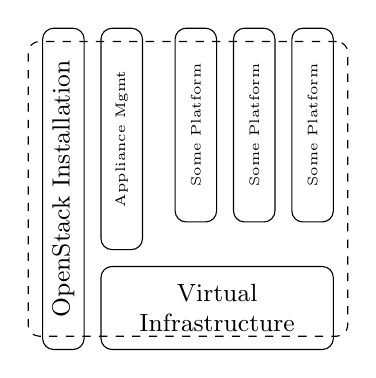
\begin{tikzpicture}[]

% cloud platform nodes
\node (cp1) [rnodesty,label={[labelsty]above:API}] {\rotatebox{90}{Some Platform}};
\node (cp2) [rnodesty,right=0.2 of cp1,label={[labelsty]above:API}] {\rotatebox{90}{Some Platform}};
\node (cp3) [rnodesty,right=0.2 of cp2,label={[labelsty]above:API}] {\rotatebox{90}{Some Platform}};

\node (ap) [rnodesty,left=0.4 of cp1.north west,anchor=north east,minimum height=8em,label={[labelsty]above:API}] {\rotatebox{90}{Appliance Mgmt}};

\path let \p1=(ap.west),\p2=(cp3.east)in
      node (virtual) [nodesty,below=0.2 of ap.south west,anchor=north west,minimum width=\x2-\x1-\pgflinewidth]
           {Virtual \\ Infrastructure};

\path let \p1=(virtual.south),\p2=(ap.north) in
      node (os) [rnodesty,left=0.2 of virtual.south west,anchor=south east,minimum height=\y2-\y1-\pgflinewidth]
           {\rotatebox{90}{OpenStack Installation}};

\node (dc) [fitsty,fit=(os.south west) (cp3.north east),inner ysep=-.5em] {};

\end{tikzpicture}
\end{document}
